\documentclass{article}
\usepackage{graphicx}

\begin{document}

%-------------------------------------------------------------------------------
%    TITLE PAGE
%-------------------------------------------------------------------------------

\begin{titlepage}
\newcommand{\HRule}{\rule{\linewidth}{0.5mm}}
\center
\textsc{\LARGE Imperial College London}  \\[1.5cm]
\textsc{\Large Department of Computing}  \\[0.5cm]
\textsc{\large Third Year Individual Project} \\[0.5cm]

\HRule \\[0.6cm]
{\huge \bfseries LOST: \\The LOgic Semantics Tutor} \\[0.3cm]
\HRule \\[1.5cm]

\begin{minipage}{0.4\textwidth}

% author
\begin{flushleft} \large \emph{Author:} \\
Alina  \textsc{Boghiu}
\end{flushleft}

% supervisors
\end{minipage}~
\begin{minipage}{0.4\textwidth}

\begin{flushright} \large \emph{Supervisor:} \\
Ian \textsc{Hodkinson}
\end{flushright}

\begin{flushright} \large \emph{Second marker:} \\
Fariba \textsc{Sadri}
\end{flushright}

\end{minipage}\\[4cm]

{\large \today}\\[3cm]
\vfill
\end{titlepage}

%-------------------------------------------------------------------------------

% What is the problem?
% Why is it interesting?
% What’s your main idea for solving it?
\section{Introduction}		% 1-3 pages

First order logic is a powerful tool, of great importance in computing and mathematics. For students it is a way of practicing and developing important logical skills and it provides a formal mean for studying and understanding common mathematical structures. However it is difficult for most students to learn the semantics of first order logic and with this being the key to assigning a truth value to any first-order logical sentence, the issue is important.\\

\noindent On the current market, there are a considerable number of tools designed to help teach natural deduction or equivalances, but very few attempts have been made to design something that will acompany the student in learning the semantics of first order logic. Feedback is currently restricted to lectures and tutorials which means this kind of instant guidance provided by computer software would make a great impact in the way students learn, improving both their and the teacher's experience. Designing such a tool raises interesting questions of what would make an interface intuitive and what does it need to provide the user with, such that they can learn and experiment with the semantics of first order predicate logic. From the actual content point of view it would be useful if the user could visualize structures in such a way that they could easily guess the meaning of a possible sentence within it. They should be able to use a toolbox-like signature to add and remove objects and relations as well as have a way of introducing and evaluating sentences. From the software development poit of view arise questions of platform compatibility, graphic interface packages, database handling, storing format etc. Overall it makes for an interesting task with numerous possible extensions.\\

\noindent The idea of a LOgic Semantics Tool (LOST) might sound simple but it is not easy to implement in an attractive way. The risk of making yet another slightly interactive tutorial is quite high therefore my aproach was to make sure this tool engages the student fully, whilst somehow motivating them to try and practice with it as much as they would with any computer game. This shaped the main idea for tackling the problem into designing a computer game where the user is assigned an avatar of his choice which they then have to train into mastering first order logic semantics. Their treinee can then complete small to complex logical missions like recognising the validity of a sentence or playing Hintikka game for which they will be awarded points. In a successful implementation a highscore database will be maintained. Finally, aquiring these points could be set as an assignment by lecturers and other further uses could be implemented.\\

\noindent The main purpose of this tool remains the most important. A minimum viable program, which allows the user to write and play around with structures, would still be a great addition to any logic student's tools. In the following sections I will explain exactly what the software wants to achieve, what stage it is at and the plan and timetable I will follow towards my final implementation.

%-------------------------------------------------------------------------------
%		Background
%-------------------------------------------------------------------------------
\section{Background}

\subsection{First order predicate logic and its semantics}

In order to understand the product I am aiming for we should first take a look at what first order predicate logic is and why its semantics can be tricky. As an extension of propositional logic, it expreses statements like \emph{Socrates is a man} in much more detail. While propositional logic would regard such a sentence as atomic and assign it a truth value, predicate logic provides a way of describing its internal structure and evaluating it inside a context. It does this by introducing:

	\begin{itemize}
	\item \emph{Constants} - which name the objects (or terms) inside a context (e.g. Socrates)
	\item \emph{Relations} - which describe properties of the objects they take as arguements or just general properties of the structure if they are nullary (i.e. take no arguements) (e.g \emph{man} is a unary relation)
	\end{itemize}.

\noindent These elements form the signature of a structure (the technical term for the context we need in order to evaluate a logic formula and asign it a truth value). For a computer scientist it may be easier to understand that the structure contains instances of the signature's elements, as well as other objects, which one can iterate over with variables. With these concepts we can now rewrite the sentence as \emph{man(Socrates)}. We now must ask two questions: Which is the object that Socrates describes and what does it mean for something to be a man. If we take our structure to be an imaginary world of dwarfs and name one of them Socrates, our sentence would be false. However in the context of the real world where everyone is human and Socrates refers to the famous philosopher, the sentence is true.\\

\noindent Next, if we want to express \emph{All men are mortal} we must introduce the two quantifiers:

	\begin{itemize}
	\item \emph{∃ (Exists)} - which checks that there is at least one object in the structure to make the sentence it refers to true.
	\item \emph{∀ (For all)} - which checks that all of the objects in the structure satisfy the sentence it refers to.
	\end{itemize}.

\noindent Now the sentence can now be written as \emph{$\forall$(men(x) $\rightarrow$ mortal(x))} and we refer to x as a variable which in this case is bound by the for all quantifier. Another aspect that the user must understand is that sentences that contain unbound variables are valid but cannot be evaluated to a truth value.\\

\noindent A good product would offer a way of visualising all of this and allow the user to play around with structures and senteces in order to better understand the semantics of first order predicate logic.

%-------------------------------------------------------------------------------
\subsection{Previous Work}
Previous attempts have been made to fill this gap in the market. The first one that came to mind was the solution one student provided for this same project specification in 2007. They developed a Java application which meets the minimum requirements and provides a few extrafeatures like the Hintikka game and an attempt at Logic-English translation. This LOST tool allowes users to enter signatures, structures and sentences, then evaluate them. It is quit eintuitive to use but it requires a fair amount of patience to get used to. This derived my decision to pay particular attention to the user experience and aim for software that one can seeminglessly learn. One particular idea came from the step by step approach to requesting input from the user for a new signature. Although the dialog box makes input easy to interpret and is a good way of creating a new signature, it means the user must already know and understand signatures. The idea was there should be a way of automatically generating the signature from an inputed sentence such that the user is pointed in the right direction. This will be further explained in the implementation details section.\\

\noindent Other application which was interesting to look at is Tarski's World. It alowes users to build three-dimentional wolrds and describe them using first order predicate logic. The chess board like environment gave me the idea of adding game like features to make the software more appealing and ejoyable. 

%-------------------------------------------------------------------------------
\subsection{The Hintikka game}
There has always been a strong link between logic and games. Ever since Aristotle they have been widely used for teaching and testing logic. The hintikka game is one very good way of understanding both the structure of a sentence and the evaluation process. It involves two players, a logic sentence and a structure. One of the players represents $\exists$ and tries to make the sentence true whilst the other represents $\forall$ and tries to make it false. The game follows the sentence's tree and I will try and implement a good winning algorithm such that the user can play against the computer.  

%-------------------------------------------------------------------------------
%  Implementation details
%-------------------------------------------------------------------------------
\newpage
\section{The LOST application: implementation details}

\subsection{General description}

\noindent The main purpose of LOST will be to model a visual representation of a structure that is intuitive to understand and easy to manipulate. Below is a picture of roughtly how the example discussed in the background section would look like. However this is only a prototype at this stage.\\

\begin{figure}[h]
\centering
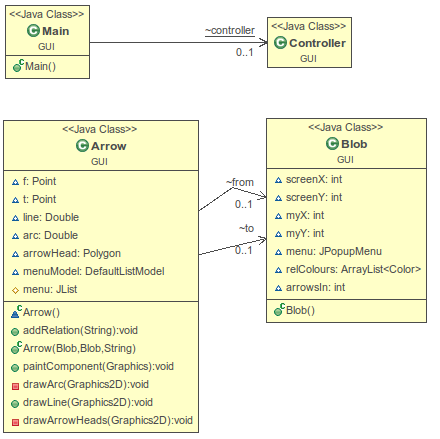
\includegraphics[width=\textwidth]{gui.png}
\caption{A structure generated by the input sentence \emph{man(Socrates)} then modified by the user, and a possible structure}
\end{figure}

\noindent The main window (the top left area) contains the structure built with elements from the signature on the right handside. At the bottom the user can input sentences for evaluation. Finally, on the right of the avatar there is a summary of the users activity.\\

\noindent In order to evaluate the sentence \emph{man(Socrates)} you should try and find the object described by Socrates and verify whether the unary relation \emph{man} applies to it. Objects will be represented by circles filled with different colours, according to which unary relations apply to it. If a constant describes an object then that object will also contain the constant's name. Looking at the signature you can see the relation \emph{man} is red. This means all the objects which it applies to will contain this colour. So it should now then easy to see that wheather our sentence is true in this context, just by finding a blue circle labeled Socrates. Finally, The binary relations will be represented by arrows from the first to the second arguement of the relation.

\noindent The User should be able to modify the structure as well as the signature. The \emph{Add New Object} button will add new circles, by default black to represent that they are not ground. The user should also be able to save the structure along with its signature as well as to load predefined ones. \\

\subsection{Progress so far}

One of the first steps when starting the implementation was choosing the main programming language. I took into consideration several facts: I am aiming for quite a complex user interface, I want to develop a desktop application compatible with most platforms to satisfy the various preferences of computing studens and the limited amount of time suggests I should pick a language I am very comfortable with. For these reasons I decided to use Java on the Netbeans IDE which provides a helpful Swing GUI builder.

	\begin{enumerate}
	\item The parser: \\
This was the first tool I worked on. Having the experience of MAlice from the previous academic year, I decided to use Antlr to generate the parser for first order logic sentences. ANTLR (ANother Tool for Language Recognition) is a powerful parser generator for reading, processing, executing, or translating structured text or binary files. From a grammar, ANTLR generates a parser that can build and walk parse trees. At this point I decided the GUI should provide the user a means of easily entering these sentences which would then be passed through to the parser in the form of a string object. I then proceeded to writing the grammar. Another choice was to use the latest version of Antlr, version 4, for its new adaptive parsing strategy which allowes a more relaxed grammar (it accepts even left recursive grammars, except for indirectly left recursive grammars where x calls y which calls x). When writing the grammar I made sure the presidence of operators is taken into account when bulding the parse tree. The Parser also checks that brackets are correctly placed and overall leaves no room for ambiguity. 

	\item The Logic Tree structure \\
The parse tree is not a neat way of storing the input sentence. It is hard to read and evaluate. Therefore I decided to build my own structure, purposely built for logic trees, in order to make the evaluation process clear and also provide a way of displaying nice trees to the user at their request.The main class is LogicTree. Here is a description of the most important elements inside it:\\

\begin{verbatim}
public class LogicTree {

    LogicTreeNode head;					
    Signature signatureBuilder;
        \\Keeps track of all the objects and relations that
          occur during the build of the logic tree and
          stores them such that a relevant signature can be
          automatically generated for the input sentence.


    public LogicTree(ParseTree c) {  
        \\Builds the logic tree from the parse tree
          generated by the parser
	    ...
	}

    evaluate(Structure s) throws UnboundException {
        \\Evaluates the tree representing the input sentence, 
          from the top down, according to the evaluation rules 
          in each node and according to the given structure.

          return head.evaluate(s);
    }
...
}

\end{verbatim}

\noindent The LogicTreeNode is the abstract class, contaning declarations of a name field of type String, an evaluation function of type boolean, which takes a structure as its parameter and a addToSignature method of type Signature that also takes a Signature as its parameter in order to add anything relevant to it. LogicTreeNode is implemented by the following classes:

	\begin{itemize}
	\item LogicTreeNotNode: Representing the unary operation not, its evaluation function returns the negated value of it's subtree.
	\item LogicTreeNullaryRelNode: Representing a nullary relation, it contains a relation field of type NullaryRel and its evaluate function returns whether that relation is true in the given structure
	\item Unary relation: LogicTreeUnaryRelNode: Similarly, contains a relation field of type Unaryl
	\item Binary operation: LogicTreeBinOpNode: Similarly, contains a relation field of type BinaryRel
	\item LogicTreeExistsNode: Representing the $\exists$ quantifier, it contains a field of type Variable and sets that variable's \emph{existsBound} field to true, the returns the truth value of its subtree
	\item LogicTreeForallNode: Similarly, sets its variable's \emph{forallBound} field to true
	\item LogicTreeEqualsNode: Represents the equals operator and has a field for each term it refers to
	\item LogicTreeTruthNode: Represents Truth and evaluates to true. It is a leaf node
	\item LogicTreeFalsityNode: Similarly, it represents Falsity.
	\end{itemize}

\noindent The quantifier and operator nodes also contain a field \emph{next} of type LogicTreeNode in order to keep track of their subtree. The rest are leaf nodes.\\

\noindent The data types mentioned above are represented by the following classes:
	\begin{itemize}
	\item Arguement: an abstract class to represent the terms that unary and binary relations refer to.
	\item Constant and Variable: implementations of Arguement. Worth mentioning are the two boolean fields inside Variable \emph{forallBound} and \emph{existBound}, that will make it easy to keep track of quantifiers.
	\item NullaryRel: with a boolean field \emph{value} that will be used to evaluate it
	\item UnaryRel : keeps track of the arguement of that relation and provides an evaluation function.
	\item BinaryRel : keeps track of both arguements and provides an evaluation function.
	\item Structure : it contains all the relations and objects that occur in the the upper left area of the screen. This is empty at first and is modified by the user through the interface. It's fields are are array lists of each of the other types.
	\item Signature : it contains all the relations and constants that occur in the user inputed sentence in the for of array lists. These are automatically generated and can be accessed through the Signature toolbox on the right side of the window and edited.
	\item BinOp: an enum type representing the binary operators and the rules to evaluate them.
	\end{itemize}

\noindent Finally, I implemented an UnbounException class that will be thrown when an unbound variable is detenced in a sentence and notifies the user of the undecidable nature of the input.

	\item The inputed logic formula:
The logic sentence is what generates the entire process of evaluation. It is inputed by the user from the keybord and with the help of the special symbols buttons provided by the interface. The standard notation is accepted. A sentence (or formula) will be composed of the following elements:

		\begin{enumerate}
		\item Atomic formulas: n-ary relations (e.g. man(Socrates) is an atomic formula), $\top$, $\bot$ or an equality (e.g. Socrates = Platon).
		\item Logic operators: $\lnot$, $\land$, $\lor$, $\to$, $\leftrightarrow$, =
		\item Quantifiers: $\forall$, $\exists$
		\end{enumerate}

Say A and B are formulas, then so are ($\lnot$ A), (A $\land$ B), (A $\lor$ B), (A $\to$ B), (A $\leftrightarrow$ B), ($\forall$ A) and ($\exists$ A). Nothing else is a formula.\\

In order to better understand the evaluation process of these formulas we should walk through our simple example: man(Socrates).
	\end{enumerate}

%-------------------------------------------------------------------------------
%     Plan and timetable
%-------------------------------------------------------------------------------
\newpage
\section{Project Plan and Timetable}		% 1-2 pages
So far I have described what a minimally viable product should do and some of the extensions I want to implement. In order to achieve this it is important to prioritise the implementation of some features and lay out a plan and timetable for the approach. Having the parser and tree structure in place, below is my timetabled plan of the remaining 11 weeks of available time for this project and a more detailed description of the features I still have to implement.

	\begin{itemize}
	\item \textbf{week 1}\\
Test and finalize this stage of the project. LOST must be able to correctly parse a sentence, generate the LogicTree from the ParseTree and evaluate it. It must also generate the structure from the inputed sentence. At this stage the structure will be inputed manually for testing purposes.
	\item \textbf{week 2}\\
Implement the structure part of the interface.
	\item \textbf{week 3}\\
Enable the loading and storing in a database of the java objects created.
	\item \textbf{week 4}\\
Allow input of multiple sentences and dinamically generate the signature such that its elements will be automatically deleted if none of the remaining sentences use them.
	\item \textbf{week 5}\\
Implement the Hintikka game.
	\item \textbf{week 6}\\
Implement the evaluation game.
	\item \textbf{week 7}\\
Adapt the interface to include the two games.
	\item \textbf{week 8}\\
Setup a user database (logins, high scores, avatars etc.)
	\item \textbf{week 9-10}\\
Testing and fixing.
	\item \textbf{week 11}\\
Finalise report and archive.
	\end{itemize}


\end{document}
